\documentclass{amsart}

\usepackage[T1]{fontenc}
\usepackage{enumerate, amsmath, amsfonts, amssymb, amsthm, thmtools, mathrsfs, wasysym, graphics, graphicx, xcolor, url, hyperref, hypcap, shuffle, xargs, multicol, overpic, pdflscape, multirow, hvfloat, minibox, accents, array, multido, xifthen, a4wide, ae, aecompl, blkarray, pifont, mathtools, etoolbox, dsfont, bbm}
\usepackage{marginnote}
\hypersetup{colorlinks=true, citecolor=darkblue, linkcolor=darkblue}
\usepackage[all]{xy}
\usepackage[bottom]{footmisc}
\usepackage{tikz}
%\usepackage{tkz-graph}
%\usepackage{tikz-qtree}
\usetikzlibrary{trees, decorations, decorations.markings, shapes, arrows, matrix, calc, fit, intersections, patterns, angles, cd}
\usepackage[external]{forest}
%\tikzexternalize
\graphicspath{{figures/}}
\makeatletter\def\input@path{{figures/}}\makeatother
\usepackage{caption}
\captionsetup{width=\textwidth}
\renewcommand{\topfraction}{1} % possibility to have one page of pictures
\renewcommand{\bottomfraction}{1} % possibility to have one page of pictures
\usepackage[noabbrev,capitalise]{cleveref}
\usepackage[export]{adjustbox}
\usepackage{ulem}\normalem

%%%%%%%%%%%%%%%%%%%%%%%%%%%%%%%%%%%%%%

% theorems
\newtheorem{theorem}{Theorem}%[section]
\newtheorem{corollary}[theorem]{Corollary}
\newtheorem{proposition}[theorem]{Proposition}
\newtheorem{lemma}[theorem]{Lemma}
\newtheorem{conjecture}[theorem]{Conjecture}
\newtheorem*{theorem*}{Theorem}%[section]
\newtheorem*{proposition*}{Proposition}%[section]
\newtheorem*{conjecture*}{Conjecture}%[section]

\theoremstyle{definition}
\newtheorem{definition}[theorem]{Definition}
\newtheorem{example}[theorem]{Example}
\newtheorem{remark}[theorem]{Remark}
\newtheorem{question}[theorem]{Question}
\newtheorem{problem}[theorem]{Problem}
\newtheorem{notation}[theorem]{Notation}
\newtheorem{assumption}[theorem]{Assumption}
\newtheorem{defprop}[theorem]{Definition/Proposition}
\newtheorem{warning}[theorem]{Warning}
\crefname{notation}{Notation}{Notations}
\crefname{problem}{Problem}{Problems}
 
% math special letters
\newcommand{\R}{\mathbb{R}} % reals
\newcommand{\N}{\mathbb{N}} % naturals
\newcommand{\Z}{\mathbb{Z}} % integers
\newcommand{\C}{\mathbb{C}} % complex
\newcommand{\I}{\mathbb{I}} % set of integers
\newcommand{\HH}{\mathbb{H}} % hyperplane
\newcommand{\K}{\mathbb{K}} % field
\newcommand{\fA}{\mathfrak{A}} % alternating group
\newcommand{\fB}{\mathfrak{S}^\textsc{b}} % signed symmetric group
\newcommand{\cA}{\mathcal{A}} % algebra
\newcommand{\cC}{\mathcal{C}} % collection
\newcommand{\cS}{\mathcal{S}} % ground set
\newcommand{\uR}{\underline{R}} % underline set
\newcommand{\uS}{\underline{S}} % underline set
\newcommand{\uT}{\underline{T}} % underline set
\newcommand{\oS}{\overline{S}} % overline set
\newcommand{\ucS}{\underline{\cS}} % underline ground set
\renewcommand{\c}[1]{\mathcal{#1}} % caligraphic letters
\renewcommand{\b}[1]{{\boldsymbol{#1}}} % bold letters
\newcommand{\bb}[1]{\mathbb{#1}} % bb letters
\newcommand{\f}[1]{\mathfrak{#1}} % frak letters
\newcommand{\h}{\widehat} % hat letters

% math commands
\newcommand{\set}[2]{\left\{ #1 \;\middle|\; #2 \right\}} % set notation
\newcommand{\bigset}[2]{\big\{ #1 \;\big|\; #2 \big\}} % big set notation
\newcommand{\Bigset}[2]{\Big\{ #1 \;\Big|\; #2 \Big\}} % Big set notation
\newcommand{\setangle}[2]{\left\langle #1 \;\middle|\; #2 \right\rangle} % set notation
\newcommand{\ssm}{\smallsetminus} % small set minus
\newcommand{\dotprod}[2]{\left\langle \, #1 \; \middle| \; #2 \, \right\rangle} % dot product
\newcommand{\symdif}{\,\triangle\,} % symmetric difference
\newcommand{\one}{\b{1}} % the all one vector
\newcommand{\eqdef}{\mbox{\,\raisebox{0.2ex}{\scriptsize\ensuremath{\mathrm:}}\ensuremath{=}\,}} % :=
\newcommand{\defeq}{\mbox{~\ensuremath{=}\raisebox{0.2ex}{\scriptsize\ensuremath{\mathrm:}} }} % =:
\newcommand{\simplex}{\b{\triangle}} % simplex
\renewcommand{\implies}{\Rightarrow} % imply sign
\newcommand{\transpose}[1]{{#1}^t} % transpose matrix

% operators
\DeclareMathOperator{\conv}{conv} % convex hull
\DeclareMathOperator{\vect}{vect} % linear span
\DeclareMathOperator{\cone}{cone} % cone hull
\DeclareMathOperator{\inv}{inv} % inversions
\DeclareMathOperator{\ninv}{ninv} % inversions
\DeclareMathOperator{\Ima}{Im} % image
\DeclareMathOperator{\Vol}{Vol} % (mixed) volume
\DeclareMathOperator{\Hom}{Hom} % hom-spaces
\DeclareMathOperator{\Ext}{Ext} % extensions

% others
\newcommand{\ie}{\textit{i.e.}~} % id est
\newcommand{\eg}{\textit{e.g.}~} % exempli gratia
\newcommand{\Eg}{\textit{E.g.}~} % exempli gratia
\newcommand{\apriori}{\textit{a priori}} % a priori
\newcommand{\viceversa}{\textit{vice versa}} % vice versa
\newcommand{\versus}{\textit{vs.}~} % versus
\newcommand{\aka}{\textit{a.k.a.}~} % also known as
\newcommand{\perse}{\textit{per se}} % per se
\newcommand{\ordinal}{\textsuperscript{th}} % th for ordinals
\newcommand{\ordinalst}{\textsuperscript{st}} % st for ordinals
\definecolor{darkblue}{rgb}{0,0,0.7} % darkblue color
\definecolor{green}{RGB}{57,181,74} % darkblue color
\definecolor{violet}{RGB}{147,39,143} % darkblue color
\newcommand{\darkblue}{\color{darkblue}} % darkblue command
\newcommand{\defn}[1]{\textsl{\darkblue #1}} % emphasis of a definition
\newcommand{\para}[1]{\smallskip\noindent\uline{#1.}} % paragraph
\renewcommand{\topfraction}{1} % possibility to have one page of pictures
\renewcommand{\bottomfraction}{1} % possibility to have one page of pictures
%\renewcommand\labelitemi{$\diamond$} % redefine itemize default symbol

% marginal comments
\usepackage{todonotes}
\newcommand{\vincent}[1]{\todo[color=blue!30]{\rm #1 \\ \hfill --- V.}}
\newcommand{\asilata}[2][]{\todo[size=\scriptsize, color=orange!30,#1]{\rm #2 \\ \hfill --- A.}}

% lattices
\newcommand{\meet}{\wedge} % meet
\newcommand{\join}{\vee} % join
\newcommand{\bigMeet}{\bigwedge} % meet
\newcommand{\bigJoin}{\bigvee} % join
\newcommandx{\projDown}[1][1={}]{\smash{\pi_\downarrow^{#1}}} % down projection map
\newcommandx{\projUp}[1][1={}]{\smash{\pi^\uparrow_{#1}}} % up projection map
\newcommand{\con}{\mathrm{con}} % congruence

% geometry
\newcommandx{\Fan}[1][1=D]{\mathcal{F}_{#1}} % fan
\newcommand{\polytope}[1]{\mathds{#1}} % font polytope

% specific wiggly
\newcommandx{\arc}[1][1=\alpha]{\b{#1}} % arc
\newcommand{\extendedWigglyComplex}{\overline{\mathrm{WC}}} % wiggly complex
\newcommand{\reducedWigglyComplex}{\mathrm{WC}} % wiggly complex
\newcommand{\wigglyFlipGraph}{\mathrm{WFG}} % wiggly flip graph
\newcommand{\wigglyIncreasingFlipGraph}{\mathrm{WIFG}} % wiggly increasing flip graph
\newcommand{\wigglyLattice}{\mathrm{WL}} % wiggly lattice
\newcommand{\wigglyFan}{\mathrm{WF}} % wiggly fan
\newcommand{\wigglyhedron}{\polytope{W}} % wigglyhedron
\newcommand{\Asso}{\polytope{A}\mathsf{sso}} % associahedron

% formating the table of contents
\setcounter{tocdepth}{4}
\makeatletter
\def\l@part{\@tocline{1}{8pt}{0pc}{}{}}
\def\l@section{\@tocline{1}{4pt}{0pc}{}{}}
\makeatother
\let\oldtocpart=\tocpart
\renewcommand{\tocpart}[2]{\sc\large\oldtocpart{#1}{#2}}
\let\oldtocsection=\tocsection
\renewcommand{\tocsection}[2]{\bf\oldtocsection{#1}{#2}}
\let\oldtocsubsubsection=\tocsubsubsection
\renewcommand{\tocsubsubsection}[2]{\quad\oldtocsubsubsection{#1}{#2}}

%%%%%%%%%%%%%%%%%%%%%%%%%%%%%%%%%%%%%%

\title{Wigglyhedra for planar point sets}

\thanks{AB was partially supported by the Australian Research Council grants DE240100447 and DP240101084. 
VP was partially supported by the Spanish project PID2022-137283NB-C21 of MCIN/AEI/10.13039/501100011033 / FEDER, UE, by the Spanish--German project COMPOTE (AEI PCI2024-155081-2 \& DFG 541393733), by the Severo Ochoa and María de Maeztu Program for Centers and Units of Excellence in R\&D (CEX2020-001084-M), by the Departament de Recerca i Universitats de la Generalitat de Catalunya (2021 SGR 00697), and by the French--Austrian project PAGCAP (ANR-21-CE48-0020 \& FWF I 5788).}

\author[D. Alcantara]{David Alcantara}
\address[David Alcantara]{Universidad de Cantabria, Santander, Spain}
\email{david.alcantara@unican.es}
%\urladdr{\url{}}

\author[A. Bapat]{Asilata Bapat}
\address[Asilata Bapat]{The Australian National University, Canberra, Australia}
\email{asilata.bapat@anu.edu.au}
\urladdr{\url{https://asilata.github.io}}

\author[M. Bin]{Marguerite Bin}
\address[Marguerite Bin]{Université de Lorraine, CNRS, INRIA, LORIA, Nancy, France}
\email{marguerite.bin@inria.fr}
%\urladdr{\url{}}

\author[N. Crepeau]{Natasha Crepeau}
\address[Natasha Crepeau]{University of Washington, Seattle, USA}
\email{ncrepeau@uw.edu}
\urladdr{\url{https://sites.google.com/view/natasha-crepeau-math/home}}

\author[H. Ping Luk]{Hoi Ping Luk}
\address[Hoi Ping Luk]{Z\'apado\v{c}esk\'a univerzita v Plzni, Pilsen, Czech Republic}
\email{hoi@connect.ust.hk}
%\urladdr{\url{}}

\author[V. Pilaud]{Vincent Pilaud}
\address[Vincent Pilaud]{Universitat de Barcelona \& Centre de Recerca Matemàtica, Barcelona, Spain}
\email{vincent.pilaud@ub.edu}
\urladdr{\url{https://www.ub.edu/comb/vincentpilaud/}}

\author[F. Santos]{Francisco Santos}
\address[Francisco Santos]{Universidad de Cantabria, Santander, Spain}
\email{francisco.santos@unican.es}
\urladdr{\url{https://personales.unican.es/santosf/}}

%%%%%%%%%%%%%%%%%%%%%%%%%%%%%%%%%%%%%%

\begin{document}

\begin{abstract}
We provide a polytopal realization of the wiggly complex of a planar point set.
\end{abstract}

\maketitle

%%%%%%%%%%%%%%%%%%%%%%%%%%%%%%%%%%%%%%

%\section{Wiggly complex and wiggly pseudotriangulations of a planar point set}
%\label{sec:wigglyComplex}
%
%\vincent{This is copy-pasted from the wigglyhedron paper. The definition is actually inexact. To be improved.}
%
%We consider an arbitrary point set~$P$ in the plane (neither necessarily aligned, nor necessarily in general position).
%
%\begin{definition}
%\label{def:wigglyComplexPointSet}
%Fix a point set~$P$ of the plane, and an arbitrary total order~$<$ on~$P$.
%A \defn{wiggly arc} is a quadruple~$(p,q,R,S)$ where~$p < q \in P$ and the sets~$R$ and~$S$ form a partition of the points of~$P$ located in the open segment joining~$p$ to~$q$.
%Two wiggly arcs~$(p,q,R,S)$ and~$(p',q',R',S')$ are \defn{crossing} if 
%\begin{itemize}
%\item either the segments~$[p,q]$ and~$[p',q']$ cross, 
%\item or~$(R \cap S') \cup (\{p,q\} \cap S') \cup (R \cap \{p',q'\}) \ne \varnothing \ne (R' \cap S) \cup (\{p',q'\} \cap S) \cup (R' \cap \{p,q\})$.
%\end{itemize}
%A set~$X$ of wiggly arcs is \defn{pointed} if for any~$p \in P$, the wiggly arcs of~$X$ with an endpoint at~$p$ generate a pointed cone.
%The \defn{wiggly complex}~$\extendedWigglyComplex_P$ is the simplicial complex of pairwise pointed and non-crossing subsets of wiggly arcs.
%Note that the boundary wiggly arcs are irrelevant, which allows us to consider a reduced wiggly complex~$\extendedWigglyComplex_P$ induced by internal wiggly arcs.
%A \defn{wiggly pseudotriangulation} of~$P$ is a facet of~$\extendedWigglyComplex_P$.
%The \defn{wiggly flip graph}~$\wigglyFlipGraph_P$ is the adjacency graph of the facets of~$\extendedWigglyComplex_P$.
%%Note that, by construction, $\wigglyFlipGraph_P$ is regular.
%See \cref{fig:wigglyComplexSquarre} for an illustration.
%%
%\end{definition}
%
%
%Observe that it is not even clear from \cref{def:wigglyComplexPointSet} that the wiggly complex~$\extendedWigglyComplex_P$ is a pure pseudomanifold (hence that the wiggly flip graph~$\wigglyFlipGraph_P$ is well-defined).
%However, we make the following ambitious conjecture.
%\vincent{The goal of this new paper is to solve this conjecture.}
%
%\begin{conjecture}
%\label{conj:polytopality}
%For any point set~$P$ in the plane, the wiggly complex~$\extendedWigglyComplex_P$ is the boundary complex of a simplicial polytope.
%\end{conjecture}
%
%In \cref{conj:polytopality}, the case of aligned points is given by the wigglyhedron of~\cite{BapatPilaud}, while the case of points in general position is given by the pseudotriangulation polytope of~\cite{RoteSantosStreinu-polytope}.
%This raises in particular the following question.
%
%\begin{question}
%Can the constructions of~\cite{BapatPilaud} be adapted to provide a more combinatorial construction of the polytope of pseudotriangulations~\cite{RoteSantosStreinu-polytope}, that would only depend on the order type (\aka oriented matroid~\cite{BjornerLasVergnasSturmfelsWhiteZiegler}) of the point configuration?
%\end{question}
%
%Using the duality between lines in the plane and points in the M\"obius strip, the pseudotriangulations of~\cite{PocchiolaVegter,RoteSantosStreinu-pseudotriangulations} were interpreted in~\cite{PilaudPocchiola} as pseudoline arrangements on sorting networks.
%It is natural to look for the analogue of this interpretation in the wiggly setting.
%
%\begin{question}
%Is there a dual interpretation of wiggly pseudotriangulations as some sort of pseudoline arrangements? 
%\end{question}
%
%This dual interpretation enables \cite{PilaudPocchiola} to consider the pseudotriangulations of~\cite{PocchiolaVegter,RoteSantosStreinu-pseudotriangulations} and the multitriangulations of~\cite{PilaudSantos-multitriangulations} under the same roof, and to define multi-pseudo-triangulations.
%The extension to the wiggly case is a natural question.
%
%\begin{question}
%Is there a multi wiggly complex?
%\end{question}
%
%Moreover, pseudoline arrangements on sorting networks can also be interpreted as (type~$A$) subword complexes of~\cite{KnutsonMiller-subwordComplex}, which in turn extend to arbitrary finite Coxeter group.
%See \cite{Stump, CeballosLabbeStump} for the study of subword complexes corresponding to cluster complexes and multi-cluster complexes.
%
%\begin{question}
%Can the wiggly complex be extended to arbitrary finite Coxeter groups?
%\end{question}
%
%%\begin{question}
%%\begin{itemize}
%%\item Is there a dual interpretation of wiggly pseudotriangulations as some sort of pseudoline arrangements? 
%%\item Is there a multi wiggly complex?
%%\item Can this interpretation be extended to other finite Coxeter groups?
%%\end{itemize}
%%\end{question}
%
%Finally, it is natural to consider the extension of~\cite[Conj.~44]{BapatPilaud}.
%
%\begin{question}
%\label{qu:Hamiltonian}
%Is the wiggly flip graph~$\wigglyFlipGraph_P$ Hamiltonian for any point set~$P$ in the plane?
%\end{question}

%%%%%%%%%%%%%%%%%%%%%%%%%%%%%%%%%%%%%%

\section{Wiggly complex}
\label{sec:wigglyComplex}

Throughout this paper, we consider an arbitrary point set~$P$ in the plane~$\R^2$ (neither necessarily aligned, nor necessarily in general position).
A point~$p \in P$ is \defn{extremal} if it is a vertex of the convex hull of~$P$.
We denote by~$n = v + w$ the number of points of~$P$, where~$v$ are extremal and~$w$ are not.
We first define the wiggly segments of~$P$.
Intuitively, a wiggly segment is like a segment~$[p,q]$ between two points~$p, q \in P$, except that the path locally deviates to one side or the other of every point in the open interval~$]p,q[$.

\begin{definition}
\label{def:wigglySegments}
An \defn{oriented arc} from~$p$ to~$q$ is an isotopy class of continuous maps~$\alpha : [0,1] \mapsto \R^2$ such that~$\alpha(0) = p$, $\alpha(1) = q$ and~$\alpha(]0,1[) \subseteq \R^2 \ssm P$.
%We say that~$p$ and~$q$ are the \defn{endpoints} of~$\arc$, and that $\arc$ is \defn{incident} to $p$ and~$q$.
An \defn{arc} is an oriented arc modulo reorientation.
An arc is \defn{internal} if its interior intersects the convex hull of~$P$, and \defn{external} otherwise.
The \defn{length} of an arc is the infimum of the lengths of the representatives in its isotopy class.
A \defn{wiggly segment} is an arc whose length is the Euclidean distance between its endpoints.
\end{definition}

\begin{definition}
\label{def:compatible}
A set~$D$ of wiggly segments is
\begin{itemize}
\item \defn{non-crossing} if there exists a set of representatives of the arcs of~$D$ with pairwise disjoint relative interiors,
\item \defn{pointed} if for any point~$p \in P$, the set of points~$q \in Q$ so that~$D$ contains a wiggly segment with endpoints~$\{p,q\}$ is contained in an open half-space at~$p$,
\item \defn{compatible} if it is both non-crossing and pointed.
\end{itemize}
\end{definition}

\begin{definition}
\label{def:wigglyDissection}
A \defn{wiggly dissection} of~$P$ is a compatible set~$D$ of wiggly segments of~$P$ containing all external wiggly segments.
\end{definition}

\begin{definition}
\label{def:wigglyComplex}
The \defn{wiggly complex}~$\reducedWigglyComplex_P$ is the simplicial complex of compatible subsets of internal wiggly segments on~$P$.
%The \defn{reduced wiggly complex}~$\reducedWigglyComplex _P$ (resp.~\defn{extended wiggly complex}~$\extendedWigglyComplex_P$) is the simplicial complex of compatible subsets of internal (resp.~of all) wiggly segments on~$P$.
See \cref{fig:wigglyComplexSquarre}\,(left).
%
\begin{figure}[!h]
\centerline{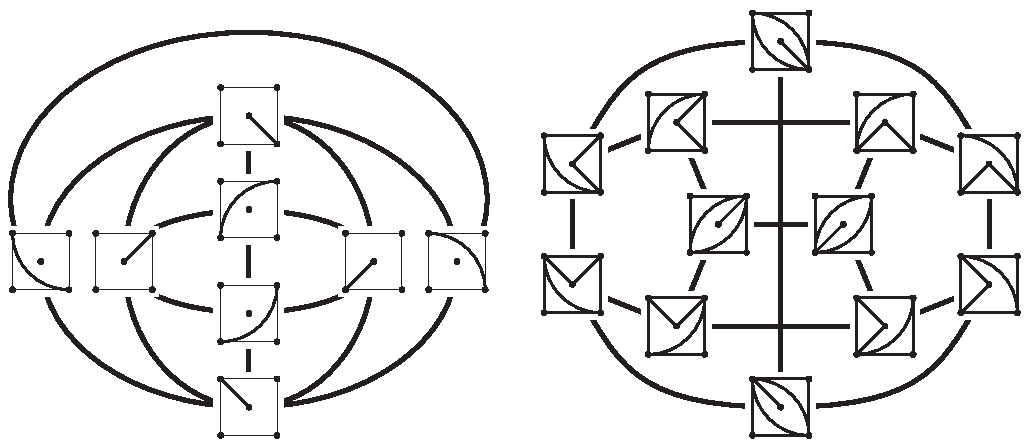
\includegraphics[scale=.85]{wigglyComplexSquare.pdf}}
\caption{The wiggly complex~$\extendedWigglyComplex_P$ (left) and wiggly flip graph~$\wigglyFlipGraph_P$ (right) of a point set~$P$.}
\label{fig:wigglyComplexSquarre}
\end{figure}
%
\end{definition}

\begin{remark}
A few observations about \cref{def:wigglySegments,def:compatible,def:wigglyDissection,def:wigglyComplex}:
\begin{enumerate}
\item The wiggly segments could also be encoded by quadruples~$(p, q, L, R)$ with~$p,q \in P$ and~$L \sqcup R  = {]p,q[} \cap P$, modulo reorientation~$(p, q, L, R) \sim (q, p, R, L)$, and the non-crossing and pointedness conditions are then purely combinatorial (see~\cite{BapatPilaud}). In this paper, we find it more intuitive and convenient to define and visualize wiggly arcs and the wiggly complex in terms of isotopy classes of arcs.
\item As the $v$ external wiggly segments are compatible with any other wiggly segments, it is convenient to ignore them in the definition of the wiggly complex~$\reducedWigglyComplex_P$, but to include them in all wiggly dissections.
In other words, the \defn{extended wiggly complex}~$\extendedWigglyComplex_P$, defined as the simplicial complex of compatible subsets of all wiggly segments on~$P$, is a $v$-fold cone over the wiggly complex~$\reducedWigglyComplex_P$.
\item \cref{def:compatible,def:wigglyDissection,def:wigglyComplex} were already largely studied in two specific situations. Namely, we refer to~\cite{BapatPilaud} for the case of aligned points, and to the original article of~\cite{PocchiolaVegter} and to the survey~\cite{RoteSantosStreinu-pseudotriangulations} for the case of points in general position.
\end{enumerate}
\end{remark}

%The following statement, known for aligned points in~\cite{BapatPilaud} and for points in general position in~\cite{PocchiolaVegter,RoteSantosStreinu-pseudotriangulations}, was extended in~\cite[Coro.~3.21]{BapatDeopurkarLicata} to the general case.
%
%\begin{theorem}[{\cite[Coro.~3.21]{BapatDeopurkarLicata}}]
%%The extended (resp.~reduced) wiggly complex~$\extendedWigglyComplex_P$ (resp.~$\reducedWigglyComplex_P$) is a simplicial ball (resp.~sphere) of dimension~$2n-3$ (resp.~$v+2w-3$).
%The wiggly complex~$\reducedWigglyComplex_P$ is a simplicial sphere of dimension~$v+2w-3$.
%\end{theorem}

The goal of this paper is to prove the following statement, already proved for aligned points in~\cite{BapatPilaud} and for points in general position in~\cite{RoteSantosStreinu-polytope}.

\begin{theorem}
\label{thm:polytope}
The wiggly complex~$\reducedWigglyComplex_P$ is isomorphic to the boundary complex of a simple polytope of dimension~$v+2w-3$.
\end{theorem}

\cref{thm:polytope} implies in particular that~$\reducedWigglyComplex_P$ is a simplicial sphere of dimension~$v+2w-4$, a result independently established in~\cite[Coro.~3.21]{BapatDeopurkarLicata}.
Note that their proof proceeds via a deformation argument, describing how the wiggly complex varies under a small perturbation of the point set.
By contrast, our approach gives a direct polytopal realization, but it depends on the fact that the wiggly complex~$\reducedWigglyComplex_P$ is a simplicial pseudomanifold without boundary of dimension~$v+2w-4$.
We thus  sketch a direct proof of this fact, both to avoid reliance on~\cite[Coro.~3.21]{BapatDeopurkarLicata} and because we believe it offers useful geometric and combinatorial insight into the structure of the wiggly complex.

\begin{definition}
Consider a wiggly dissection~$D$ of~$P$ (we actually implicitly consider a set of pairwise non-crossing representatives of the arcs of~$D$).
The arcs of~$D$ separate the plane~$\R^2$ into connected components, whose closure we call \defn{wiggly cells}.
We call \defn{external} cell the one outside the external wiggly arcs, and \defn{internal} all other cells.
Note that each internal wiggly cell~$C$ has an external boundary component (separating it from the external cell), and may have some internal boundary component.
The \defn{corners} of~$C$ are the convex vertices along its boundary and the \defn{chains} of~$C$ are the pieces of its boundary between two consecutive corners.
A \defn{wiggly triangle} is a wiggly cell with $3$ corners and no internal boundary.
A \defn{wiggly quadrangle} is a wiggly cell with $4$ corners and no internal boundary, or a wiggly digon with a single interior point.
\end{definition}

\begin{proposition}
Any wiggly dissection~$D$ of a set of $n$ points contains at most $2n-3$ wiggly segments and at most~$n-2$ internal wiggly cells.
Moreover, the following assertions are equivalent:
\begin{enumerate}[(i)]
\item $D$ is an inclusion maximal wiggly dissection,
\item all wiggly cells of~$D$ are wiggly triangles,
\item $D$ has $n-2$ internal wiggly cells and is connected,
\item $D$ has $2n-3$ wiggly segments.
\end{enumerate}
We then say that~$D$ is a \defn{wiggly triangulation}.
\end{proposition}

\begin{proof}[Proof sketch]
\para{(i) $\Rightarrow$ (ii)}
Consider a wiggly cell~$C$ of a maximal wiggly dissection~$D$.
Note that~$C$ has at least $2$ corners, and at least $3$ if it has no internal boundary.
Consider now an arc~$\arc$ between two corners of~$C$.
Stretch~$\arc$ until you get a geodesic~$\arc'$ inside~$C$, and cut~$\arc'$ into subarcs at the points of~$P$ it contains.
The resulting arcs are wiggly segments compatible with~$D$ (they are non-crossing with~$D$ because~$\arc$ was inside~$C$, and they are pointed with~$D$ because the endpoints of~$\arc$ are corners of~$C$).
By maximality of~$D$, it implies that all these wiggly segments already belong to~$D$.
In other words, the geodesic~$\arc$ is a chain of~$R$.
This observation implies that~$C$ has precisely $3$ corners (otherwise, we have an arc joining two non consecutive corners of~$R$, thus not isotopic to a chain of~$R$) and no internal boundary component (otherwise there is a loop at a corner of~$R$ not isotopic to a chain of~$R$).
In other words, $C$ is a wiggly triangle.

\para{(ii) $\Rightarrow$ (iii)}
Assume that all cells of a wiggly dissection~$D$ are wiggly triangles.
Note that this implies in particular that~$D$ is connected (as otherwise some wiggly cell would have an internal connected component).
Moreover, assume that $D$ has $n$ vertices, $m$ edges, $c$ internal cells, and~$a$ angles.
Then $n-e+r=1$ (Euler's relation), $a = 2e$ (because the number of corners around each vertex is its degree) and $a = 3r + n$ (because each cell has at $3$ convex angles, and $D$ has precisely $n$ concave angles, since each vertex is pointed).
We conclude that~$e = 2n-3$ and~$r = n-2$.

\para{(iii) $\Rightarrow$ (iv)}
If~$D$ is connected and has~$n-2$ internal wiggly cells, then~$e = n + r - 1 = 2n - 3$ by Euler's relation.

\para{(iv) $\Rightarrow$ (i)}
Any wiggly dissection~$D$ is contained in an inclusion maximal wiggly dissection~$D'$.
We have shown that (i) $\Rightarrow$ (ii) $\Rightarrow$ (iii) $\Rightarrow$ (iv), so that~$D'$ has~$2n-3$ wiggly segments.
We obtain that $D$ has at most $2n-3$ wiggly segments and at most~$n-2$ wiggly cells.
Moreover, if~$D$ has $2n-3$ edges, the~$D = D'$ is inclusion maximal.
\end{proof}

\begin{proposition}
\label{prop:diagonals}
Any wiggly quadrangle~$Q$ admits precisely two wiggly diagonals, \ie wiggly segments of~$P$ inside~$Q$ and compatible with~$Q$.
\end{proposition}

\begin{proof}[Proof sketch]
If~$Q$ is a wiggly digon with a single interior point, then it contains precisely two arcs which are non crossing and not isotopic to the boundary (namely joining one of the corners to the interior point), and they are both compatible with~$Q$.
Otherwise, the diagonals of~$Q$ are the two wiggly segments in the interior of~$Q$ along the geodesics obtained by stretching the two arcs joining the two pairs of opposite corners of~$Q$.
\end{proof}

\begin{definition}
The \defn{wiggly flip graph}~$\wigglyFlipGraph_P$ of~$P$ is the graph with a vertex for each wiggly triangulation of~$P$, and with an edge between two wiggly triangulations~$T$ and~$T'$ of~$P$ if and only if there are wiggly segments~$\arc \in T$ and~$\arc' \in T'$ such that~$T \ssm \{\arc\} = T' \ssm \{\arc'\}$.
\end{definition}

\begin{proposition}
The wiggly flip graph~$\wigglyFlipGraph_P$ is regular of degree~$v+2w-3$ and connected.
\end{proposition}

\begin{proof}[Proof sketch]
Consider an internal wiggly segment~$\arc$ in a wiggly triangulation~$T$ of~$P$.
Let~$Q$ denote the wiggly quadrangle obtained by merging the two wiggly triangles incident to~$\arc$.
By~\cref{prop:diagonals}, there are precisely two wiggly segments of~$P$ inside~$Q$ and compatible with~$Q$.
This proves that~$\wigglyFlipGraph_P$ is $(v+2w-3)$-regular.

Consider now an arbitrary order~$p_1, \dots, p_n$ of~$P$ such that~$p_i$ lies on the complement of the convex hull of~$\{p_1, \dots, p_{i-1}$ for all~$i \in [n]$.
For all~$i \in [n]$, define inductively the wiggly triangulation~$T_i^\circ$ of~$P_i \eqdef \{p_1, \dots, p_i\}$ obtained from~$T_{i-1}^\circ$ by adding all external wiggly segments of~$P_i$.
We prove by induction on~$i$ that any wiggly triangulation of~$P_i$ is connected by flips to~$T_i^\circ$.
For any wiggly triangulation~$T_i$ of~$P_i$, consider the wiggly triangulation~$T_{i-1}$ obtained from~$T_i$ by flipping all internal wiggly segments incident to~$p_i$, and then deleting~$p_i$ and its two incident external wiggly arcs.
Then~$T_{i-1}$ is a wiggly triangulation of~$P_{i-1}$, which is connected by flips to~$T_{i-1}^\circ$ by induction.
We conclude that~$T_i$ is connected by flip to~$T_i^\circ$.
\end{proof}

%%%%%%%%%%%%%%%%%%%%%%%%%%%%%%%%%%%%%%

\section{Rigidity}
\label{sec:rigidity}
The normal fan of the polytope mentioned in~\cref{thm:polytope} is spanned by rigidity vectors of wiggly edges, which we now define.
First, given a wiggly arc \(\arc\) with endpoints \(p\) and \(q\) in a point set \(P\), the  points of \(P\) lying on the open segment \(]p,q[\) are called the~\defn{waypoints} of \(\arc\).

All rigidity vectors lie in \((\R^2)^P \cong (\R^2)^n\).
The rigidity vector of \(\arc\) is the combination of a longitudinal component whose every coordinate is parallel to \(\arc\), and a transversal component whose every coordinate is orthogonal to \(\arc\).
The longitudinal component is zero at any coordinate that is not an endpoint.
The transversal component is zero at any coordinate that is neither an endpoint nor a waypoint.
The longitudinal rigidity vector was used extensively in~\cite{RoteSantosStreinu-polytope} to construct a polytope in the case of points in general position.
When \(P\) is arbitrary, we need to perturb the longitudinal rigidity vector by a small multiple of the transversal rigidity vector.
We show in ??? that this procedure gives us a complete normal fan.

Given \(x \in \R^2\) and \(r \in P\), denote by \(x \mathbbm{1}_r\) or \(x \cdot \mathbbm{1}_r\) the vector in \((\R^2)^P\) that has \(x\) in the \(r\)th coordinate and zero elsewhere.
  In the following definitions, let \(\arc\) be a wiggly segment on a point set \(P\), with endpoints \(p\) and \(q\).
\begin{definition}
  The~\defn{longitudinal rigidity vector} \(R_l(\arc)\) of \(\arc\) is defined as
  \[R_l(\arc) = (p-q) \mathbbm{1}_p  + (q-p) \mathbbm{1}_q.\]
\end{definition}
For a vector \(w \in \R^2\), denote by \(w^{\perp}\) the rotation of \(w\) by \(90^{\circ}\) in the anti-clockwise direction.
\begin{definition}
  The~\defn{transversal rigidity vector} \(R_t(\arc)\) of \(\arc\) is a row vector in \((\R^2)^P\) defined as follows.
  Let \(w_1, \ldots, w_r\) be the waypoints of \(\arc\) in order from \(p\) to \(q\).
  For convenience, set \(p = w_0\) and \(q = w_{r+1}\).
  For \(i \in [1,r]\), the contribution to \(R_t(\arc)\) from \(w_i\) is the vector
  \[\mathsf{sgn} \cdot \left( - (p_{i+1} - p_i)^{\perp} \mathbbm{1}_{i-1} + (p_{i+1} - p_{i-1})^{\perp} \mathbbm{1}_i - (p_i - p_{i-1})^{\perp}\mathbbm{1}_{i+1}  \right),\]
  where \(\mathsf{sgn} = +1\) if \(\arc\) passes to the right of \(w_{i+1} - w_{i-1}\) around \(w_i\), and \(\mathsf{sgn} = -1\) otherwise.
  The vector \(R_t(\arc)\) is the sum of all these contributions for \(i \in [1,r]\).
\end{definition}
\begin{definition}
  For \(\epsilon > 0\), the~\defn{(total) \(\epsilon\)-rigidity vector} \(R^{\epsilon}(\arc)\) is defined as
  \[R^{\epsilon}(\arc) = R_l(\arc) + \epsilon R_t(\arc).\]
\end{definition}
We now assemble the rigidity vectors into rigidity matrices.
All of these have rows indexed by the wiggly arcs on \(P\).
Each row is a rigidity vector, and thus lies in \((\R^2)^P\).
\begin{definition}
  The~\defn{longitudinal rigidity matrix} of \(P\) is the matrix \(M_l(P)\) whose row indexed by \(\arc\) is \(R_l(\arc)\).
The~\defn{transverse rigidity matrix} of \(P\) is the matrix \(M_t(P)\) whose row indexed by \(\arc\) is \(R_t(\arc)\).
The~\defn{(total) \(\epsilon\)-rigidity matrix} of \(P\) is the matrix \(M^{\epsilon}(P)\) defined as \(M_l(P) + \epsilon M_t(P)\).
\end{definition}
% \begin{definition}
% The \defn{rigidity matrix} of the point set~$P \eqdef \{p_1, \dots, p_n\} \subseteq \R^2$ is the matrix~$R_P$ with $\binom{n}{2}$ rows and $2n$ columns where the $k$th pair of entries in the $(i,j)$th column contains the coordinates of~$p_i-p_j$ if $k = i$, of $pj-p_i$ if~$k = j$, and $0$ otherwise.
% \end{definition}

% \begin{definition}
% The \defn{rigidity map} and \defn{dual rigidity map} of the point set~$P \subseteq \R^2$ are the dual maps
% \[
% R : 
% \begin{array}{ccc}
% (\R^2)^P & \to & \R^{\binom{P}{2}} \\
% (v_p)_{p \in P} & \mapsto & \bigl( \dotprod{v_p-v_q}{p-q} \bigr)_{p,q \in P}
% \end{array}
% \]
% \end{definition}

%\begin{definition}
%The \defn{rigidity map} of the point set~$P \eqdef \{p_1, \dots, p_n\} \subseteq \R^2$ is the map~$R_P : (\R^2)^n \to \R^{\binom{P}{2}}$ defined by~$R \bigl( (v_p)_{p \in P} \bigr) = \bigl( \dotprod{v_p-v_q}{p-q} \bigr)_{p,q \in P}$.
%Its dual map~$R_P^* : \R^{\binom{P}{2}} \to (\R^2)^P$ is given by~$R_P^* \bigl( (c_{p,q})_{p,q \in P \bigr)$
%The kernel of~$R_P$ is the space of \defn{rigid infinitesimal motions}, and is generated by the infinitesimal translations~$(v)_{p \in P}$ and the infinitesimal rotations~$(p^\perp)_{p \in P}$ (where~$(x,y)^\perp = (-y,x)$).
%The image of~$R_P^*$ is the space of \defn{forces under equilibrium} 
%\end{definition}



%%%%%%%%%%%%%%%%%%%%%%%%%%%%%%%%%%%%%%

\section{Wigglyhedron}
\label{sec:wigglyhedron}



%%%%%%%%%%%%%%%%%%%%%%%%%%%%%%%%%%%%%%

\section{Proof}
\label{sec:proof}

%\begin{definition}
%Let $\b{R} : V \to \R^d$ be a vector configuration and~$f : V \to \R$ be a height function with the same label set~$V$.
%The \defn{coherent subdivision} of~$(\b{R}, f)$ is the projection into~$\R^V$ of the lower hull of the 
%\end{definition}

The proof relies on the following statement.

\begin{theorem}
Let~$\simplex$ be a $(d-1)$-dimensional pseudomanifold without boundary, and let~$\b{R} : V \to \R^d$ be a vector configuration and~$f : V \to \R^+$ be a height function both labeled by the vertex set~$V$ of~$\simplex$.
Then the following are equivalent:
\begin{itemize}
%\item $\simplex$ is the coherent triangulation of the vector configuration~$\b{R}$ with respect to the height function~$f$,
\item $\simplex$ is the boundary complex of the convex hull of the points~$\lambda(v) \, \b{R}(v)$ for all~$v \in V$,
\item For every minimal non-face~$F$ of~$\simplex$, there is a linear dependence~$\lambda: V \to \R$ of the vector configuration~$\b{R}$ whose negative part is~$F$ and which evaluates negatively with~$f$, that is
\[
F = \set{v \in V}{\lambda(v) < 0},
\qquad
\sum_{v \in V} \lambda(v) \, \b{R}(v) = \b{0},
\qquad\text{and}\qquad
\sum_{v \in V} \lambda(v) \, f(v) < 0.
\]
\end{itemize}
\end{theorem}

\begin{proof}
\end{proof}

The first step of the proof is thus to understand the minimal non faces of the wiggly complex~$\reducedWigglyComplex_P$.


%%%%%%%%%%%%%%%%%%%%%%%%%%%%%%%%%%%%%%

%\clearpage
\addtocontents{toc}{ \vspace{.1cm} }
\bibliographystyle{alpha}
\bibliography{wigglyhedra}
\label{sec:biblio}

\end{document}

% Local Variables:
% TeX-command-extra-options: "-pvc"
% End:
